We created the topology shown in Figure~\ref{fig:topology} in ExoGENI to conduct our experiments.  The emulated topology follows the power law, i.e., $4$ routing 
nodes in the middle to emulate the backbone domains and the rest emulate the access domains in between the backbone nodes and the end hosts. 

Among the $23$ nodes in this topology, we specify $6$ data origins and $6$ data sinks as the end hosts to transfer a batch of data files of different sizes that we randomly acquired from OSG. 
This file batch is transferred between every chosen pair of end hosts. We ran two sets of experiments to collect two sets of raw training data. In the first one, called {\it Partial},
data transfers only happen between the origins and sinks, where every origin node sends all the files in the batch 
to all the receiving nodes in parallel. In the second one, called {\it Complete}, data transfers happen between all the end host pairs. 
The file integrity is being checked at the receiving end host and each file transfer accounts for one data flow and therefore 
a data sample in a training data set. We further parallelized the data transfer process to reduce the emulation time down to about twenty-four hours for this particular network.  

For each experiment, probabilistic integrity error or network impairment via the Chaos Jungle tool is injected to the $54$ link interfaces and $12$ end hosts in sequence with the given probability setting, which 
For each fault injection scenario, the entire set of {\it Partial} or {\it Complete} data transfers are conducted. Each link interface or node component with fault injected represents a label.  
The receiving node checks if a received file is identical to its original copy via checksum and marks this data transfer as a failure data sample if checksums do not match. 
We treat retransmission as a separate feature for the data samples.  A file could also be missed at the destination due to ultimate transfer failure which is also treated as a failure. 
If the checksum matches, this data transfer becomes a success data sample in the training data set. Otherwise, it is labeled by the corresponding faulty element, one of the total $66$ labels in this study. 
The final {\it Complete} training data set consists of 8,006,592 data samples.

Through extensive training data analysis, we hope to achieve three major goals in our RCA study: (1) performance comparison in terms of accuracy and training time performance of different models, 
(2) impact quantification of different types of features on the model performance, esp. the file size and the transfer throughput, because the other features like data transfer source and destination, integrity error, 
and transfer status (retransmission, etc.) are all indispensable, (3) handling of the inherited data imbalance in the training data set. 

We compared different variants out of the three ML model families presented in Section~\ref{sec:ml} and presented the best model from each one: Random Forest, Linear SVC, and Multinomial Naive Bayes.
We use One Hot Encoding for all the categorical features. As a very basic benchmark, we note the accuracy of random classification would be merely $\frac{1}{66}$. 

Each figure shows five different performance metrics under four scenarios. The five metrics are F1 score with per-flow inference, the accuracy with per-({\it Flow}) inference, and the $Top-1$, $Top-2$, and $Top-3$ accuracy with
the {\it Aggregated Flow} inference. The four scenarios are {\it Partial} and the {\it Complete} data sets with {\it All Features} or only {\it No File features}.

\begin{figure}[!ht]
\begin{center}
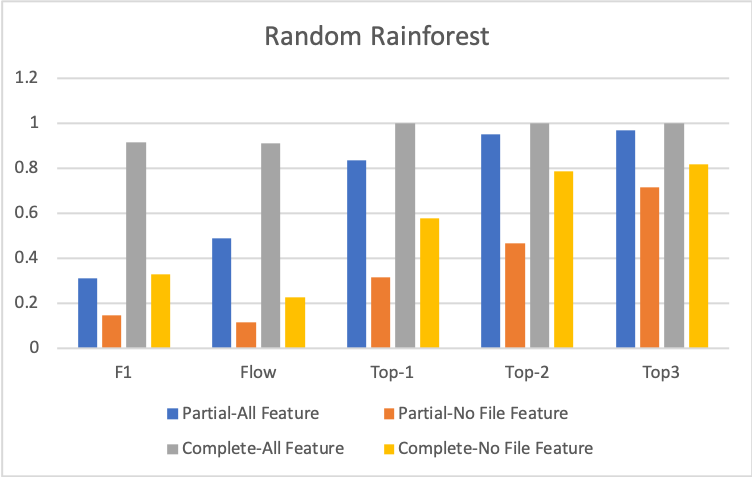
\includegraphics[width=0.45\textwidth]{./figure/rf-accuracy}
\end{center}
\caption{Classification Accuracy with Random Forest Model}
\label{fig:dt}
\end{figure}

Fig.~\ref{fig:dt} presents the results from training random forest models with different data sets. Two prominent observations stand out. 
First, it clearly shows that the model with {\it Complete} data performs significantly better than the {\it Partial} case. This illustrates the importance of sufficient 
coverage of the network path information in the training data set. It also shows that, even without the full coverage of network path between the network routers, 
the flows between end hosts along can guarantee very high RCA inference accuracy.   
Secondly, training with {\it All Features} outperforms its {\it No File Features} counterpart by a large margin. This means the file transfer statistics can boost the inference performance.  
We also learned that the file transfer throughput has a bigger impact than the file size, though the result is not shown here. 

When we zoom into more details, we can see that the combined {\it Complete-All Features} data set presents satisfactory performance even with the single flow-based testing data samples with 
both F1 score and accuracy reaching above $0.90$. When the aggregated flow data samples are used for inference, the accuracy scores perfect $1$. The next best scenario is when {\it All Features} presented with 
{\it Partial} data transfer, while the single flow-based inference only achieved under $0.5$ accuracy, the aggregated flow-based inference doubles the accuracy and quickly narrows down the root cause to the 
top $2$ elements. However, without more path coverage, it doesn't achieve perfect accuracy until $Top-10$. For the next two scenarios, the aggregated flow inference helps achieve better performance 
and {\it Complete} path coverage appears more important than the inclusion of file transfer features. However, the best it can achieve is a mere $80\%$ $Top-3$ accuracy.  

\begin{figure}[!ht]
\begin{center}
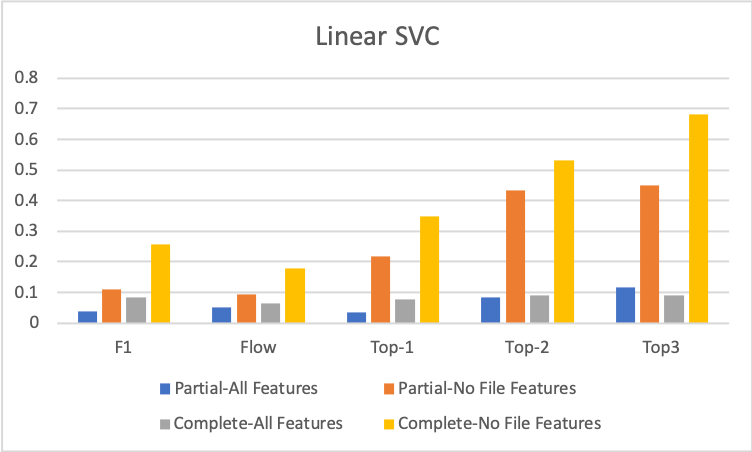
\includegraphics[width=0.45\textwidth]{./figure/svc-accuracy}
\end{center}
\caption{Classification Accuracy with SVM Model}
\label{fig:svm}
\end{figure}

Fig.~\ref{fig:svm} depicts the results using a linear SVC model. It shows the same tendency with regards to {\it Complete} file transfer coverage and the aggregated flow inference. 
However, the inclusion of file transfer features poses very negative impacts. We believe this is due to the incapability of SVM family models in dealing with mixed numerical and categorical features. 
Overall, comparing to the rain forest model, it scores much worse in every performance metric as it only obtained less than $0.7$ $Top-3$ accuracy.

\begin{figure}[!ht]
\begin{center}
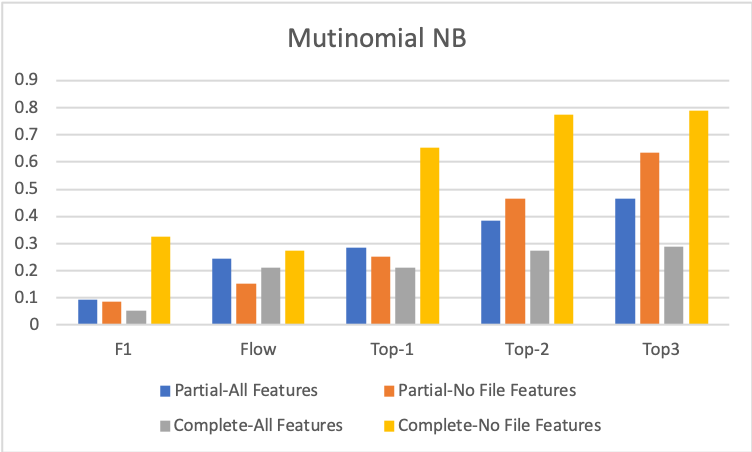
\includegraphics[width=0.45\textwidth]{./figure/nb-accuracy}
\end{center}
\caption{Classification Accuracy with Multinomial Naive Bayes}
\label{fig:bn}
\end{figure}

Fig.~\ref{fig:bn} shows the results with the Multinomial Naive Bayes model. Again, the accuracy increases with $k$. The single flow level accuracy is very poor and the accuracy increases dramatically with bigger $k$. 
It in general follows the pattern of the SVM model except it performs better in all the metrics. For example, its $Top-3$ accuracy is above $0.8$. Another difference is that, in the {\it Partial} scenario, it performs better with the {\it All-Features} than that with only {\it No File Features (NF) } for the F1-score, flow-based accuracy, and the $Top-1$ accuracy.

We next look into the training time of the above three models when using a Macbook Pro laptop with the Quad-Core i7 CPU and 16GB RAM. We note this only helps with the relative compute time performance comparison among the models since we can always use more powerful servers with larger training data set. From Table.~\ref{tab:time}, it is clear that the linear SVC model takes a substantially longer time than the other two to converge in all four cases. The SVC with the default RBF kernel takes a longer time and fails to converge after several hours even for the {\it Partial} data set which is not shown here. Between the other two, the BN model takes the shortest time (in sub-seconds) but all the training of the random forest models converge in a few seconds. The next observation is that the training with the {\it Complete} data set finishes much faster than its counterpart with {\it Partial} data set. This makes sense because more complete training data helps the model training converge faster. Due to the same reason, the data set with the {\it All Features (AF)} converges faster sometimes.

\begin{table}[!ht]
\caption{Training Time }
\label{tab:time}
%\vspace{-0.1in}
\begin{center}
\begin{tabular}{ |c|c|c|c|c| } 
 \hline
  & Partial-AF & Partial-NF & Complete-AF & Complete-NF\\ 
 \hline
 Forest & 5.45s & 2.42s & 4.23s & 1.54s\\ 
 \hline
 Bayes & 0.5s & 1.54s & 0.18s & 0.43s\\
 \hline
 SVC & 575s & 600s & 75s &70s\\ 
 \hline
\end{tabular}
\end{center}
%\vspace{-0.1in}
\end{table}
Combining both training accuracy and training time, the random forest model appears to be a clear winner for the RCA problem under our study since its trained model achieves excellent accuracy performance with rather short training time. BN models deserve further exploration due to its fast convergency and relative benign performance.

In order to gain more insight into the classification accuracy performance, we observed that the majority of mislabeled data in the classification inference are those with labels of end host faults in all the scenarios whose accuracy is less than $1$.  This is because the raw training data set is highly imbalanced due to the different impacts of the injected failures on the data files being transferred (Section~\ref{sub:ml:imbalance}). There are significantly fewer integrity errors caused by the faulty end hosts, \ie, significantly less labeled data in these classes. 

We take the {\it Complete-No File Features} data set with the Random Forest model as an example. The details are shown in Table~\ref{tab:class}. We first categorize all the labeled data into two groups: those with faulty link interfaces and those with faulty end hosts, {\it Max} and {\it Min} represent the maximum and the minimum number of samples in a class in each category and the $Top-k$ up to $k=3$ accuracy under each category is calculated separately. We can see that there are a hundred times more samples in a few link failure classes than those in all the end host failure classes, and samples from some link failures classes are about ten times less than those from some other link failure classes. As a result, all the end host failures are misclassified in all the cases, while most link failure cases are correctly classified and the accuracy reaches $1$ when $k=3$.

\begin{table}[!ht]
\caption{Classification Accuracy Differentiation}
\label{tab:class}
%\vspace{-0.1in}
\begin{center}
\begin{tabular}{ |c|c|c|c|c| } 
 \hline
  \multicolumn{5}{|c|}{Link Faults} \\
 \hline
 Max & Min & $Top-1$ & $Top-2$ & $Top-3$\\ 
 \hline
 1443 & 121  & 0.70 &  0.96 & 1 \\
 \hline
\end{tabular}

\begin{tabular}{ |c|c|c|c|c|} 
 \hline
\multicolumn{5}{|c|}{Host Faults} \\
 \hline
 Max & Min & $Top-1$ & $Top-2$ & $Top-3$ \\ 
 \hline
11 & 11  & 0 &  0 & 0\\
  \hline
\end{tabular}
\end{center}
%\vspace{-0.1in}
\end{table}

The main techniques to solve the dataset imbalance problem are to rebalance the data via oversampling or downsampling data from different classes. Since the labeled data subsets from the end host failure classes are rather small, the pure downsampling techniques will not improve on the model performance. We focus on two representative oversampling techniques: random and SMOTE as well as two methods that combine oversampling and downsampling.
These methods have been implemented in the {\it imbalanced-learn} library~\cite{imbalance-learn:web}.

The random oversampling approach is straightforward in which new samples are randomly generated by copying the existing samples from the underrepresented classes. The SMOTE (Synthetic Minority Oversampling Technique) ~\cite{smote:2002} generates new samples by interpolation rather than duplication of existing samples using variants of k-Nearest Neighbors classifier method. At the end of the oversampling with the above example, the augmented data set will have 1443 labeled data for each of the 66 classes. 

SMOTETomek is a combined method that uses SMOTE for Oversampling and removes Tomek links for downsampling. Tomek links identify two samples that are too close to each other. SMOTEENN is another popular method that combines over- and under-sampling based on SMOTE.

For the  {\it Complete-All Features} data set, our analysis indicated that both Random and combined SMOTE methods resulted in similar perfect $Top-k$ performance but slightly reduced flow-based F1 Score and accuracy. SMOTE actually deteriorated all the metrics. The observations on the  {\it Complete-No File Features} data set are similar. Since the performance of the original model is already perfect for the former case, we only present the results on the two {\it Partial} data sets.


\begin{figure}[!ht]
\begin{center}
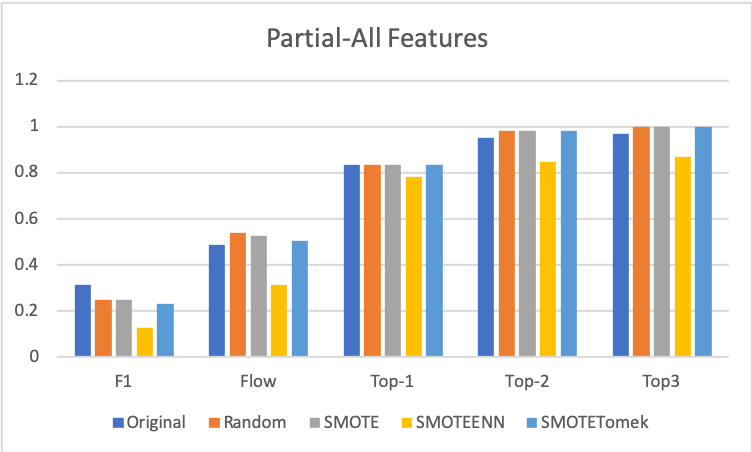
\includegraphics[width=0.45\textwidth]{./figure/partial-all-oversampling}
\end{center}
\caption{Oversampling with All Features}
\label{fig:os:all}
\end{figure}

\begin{figure}[!ht]
\begin{center}
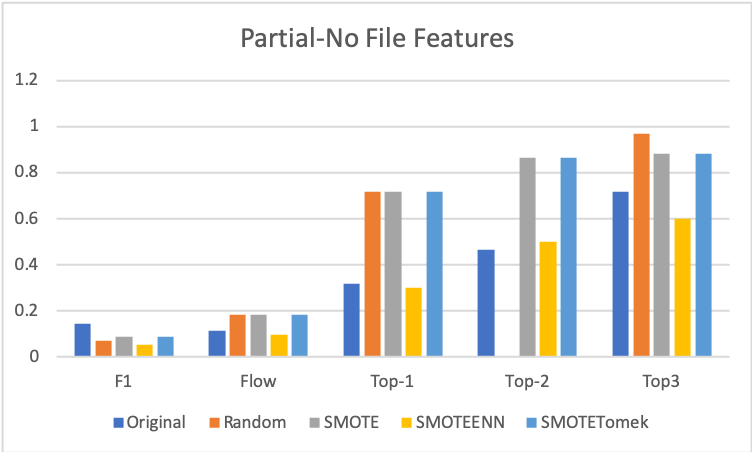
\includegraphics[width=0.45\textwidth]{./figure/partial-nofile-oversampling}
\end{center}
\caption{Oversampling with No File Features}
\label{fig:os:nofile}
\end{figure}

The results in Fig.~\ref{fig:os:all} and~\ref{fig:os:nofile} show that the SMOTEENN method doesn't help the performance. The other three all improve the performance to some extent though at different scales, especially on the $Top-k$ accuracy measurement. The basic random oversampling demonstrates the best performance improvement in most cases.  The main takeaway is that multiple sampling methods have to be carefully evaluated in order to find the best one.
